
\chapter{Desarrollo}
\label{cha:desarrollo}

\begin{FraseCelebre}
  \begin{Frase}
    Cada uno de nosotros debe trabajar para su propia mejora, y al mismo tiempo compartir una responsabilidad general para toda la humanidad.
  \end{Frase}
  \begin{Fuente}
    Marie Curie
  \end{Fuente}
\end{FraseCelebre}

\section{Introducción}
\label{sec:intro-desarrollo}

En el presente \gls{tfm} se ha desarrollado una estrategia de detección de objetos abandonados para ser aplicado en sistemas de videovigilancia. Como ya se comentó al final de la sección \ref{subsec:comparativa-detectores}, se utilizará como detector de objetos y personas \gls{yolov4} y como algoritmo de seguimiento \gls{deepsort}. A continuación, se describen las diferentes secciones que componen este capítulo.

Primero se evaluará YOLOv4 sobre Darknet, framework de código abierto escrito en C y \gls{cuda}, y se analizará la precisión y velocidad que se obtienen en la detección de objetos y personas. Posteriormente se convertirá el modelo de \gls{yolov4} de Darknet a Tensorflow, framework de código abierto escrito en Python y C++ orientado al desarrollo de algoritmos inteligentes de Machine Learning. Utilizar \gls{yolov4} con Tensorflow facilitará la programación del algoritmo de detección de objetos abandonados con Python, ya que Darknet no es un framework de uso extendido y podría ser más difícil encontrar soluciones para los posibles errores. A continuación se reentrenará el modelo de la red \gls{yolov4} sobre el dataset \gls{oidv4} para observar si se obtienen mayores valores en las métricas de calidad respecto a \gls{coco}.

Una vez obtenido el modelo de \gls{yolov4} definitivo, se probará el algoritmo de seguimiento \gls{deepsort}. Solo nos interesa la detección y seguimiento de personas y objetos de interés, por lo que se filtrará la detección para que solo se identifiquen las clases que queremos.

Finalmente, se expondrá una estrategia para la detección de objetos abandonados basada en la detección de objetos y personas mediante \gls{cnn}'s y se implementará sobre el detector de objetos \gls{yolov4} junto al algoritmo de detección \gls{deepsort}. En el planteamiento del algoritmo de detección de objetos abandonados se tendrá que considerar dos posibles escenarios. El primero es que se identifique un objeto sin propietario que se encuentre estacionario durante toda la ejecución de la secuencia de vídeo. En este caso, se emitirá una señal de alarma cuando se superen los 15 segundos del objeto inmóvil. En el segundo escenario se deberá de crear una asociación entre persona y objeto. Una vez establecida la asociación se podrá evaluar cuando una persona abandona un objeto de su propiedad a una una distancia en píxeles 5 veces mayor a la distancia a la que se encontraba en el momento que se realizó la asociación.

Cabe recalcar que en este capítulo se va a exponer cada uno de los procedimientos que se han llevado a cabo para poner en funcionamiento los algoritmos de detección, seguimiento y detección de objetos abandonados. Todos los resultados obtenidos durante el desarrollo de esta parte del proyecto se pueden consultar en el capítulo \ref{cha:resultados}.

\section{Detección de personas y objetos con YOLOv4}
\label{sec:desarrollo-yolov4}

\gls{yolov4} es un algoritmo de detección que utiliza \textit{Deep Learning} y \gls{cnn} para detectar objetos. Como lo indica su nombre solo necesita ``ver'' la imagen una sola vez, lo cual permite ser el muy rápido aunque sacrificando precisión. Esta rapidez permite detectar objetos en tiempo real.

\gls{yolov4} está originalmente implementado en Darknet, un framework de redes neuronales de código abierto escrito en C y \gls{cuda} y sirve como base de \gls{yolo}. Es rápido, fácil de instalar y admite cálculos de \gls{cpu} y \gls{gpu}. Darknet utiliza como framework para entrenar \gls{yolo}, lo que significa que establece la arquitectura de la red. El primer autor de Darknet es el autor del propio \gls{yolo} (J Redmon) y actualmente está siendo liderado por Alexey Bochkovskiy.

Para la utilización de \gls{yolov4} se ha instalado previamente la librería opencv-python 4.1.1.26 junto con \gls{cuda} 10.1.243 y cuDNN 7.6.5 para poder codificar de manera más optima los algoritmos utilizando una \gls{gpu} NVIDIA.

Se ha clonado el repositorio de \gls{yolov4} de GitHub \cite{yolov4-darknet-github} en el framework Darknet. Para obtener el máximo rendimiento por parte del equipo que se está utilizando se ha modificado el fichero Makefile para habilitar la utilización de la \gls{gpu} junto con \gls{cuda}, así como OpenCV para poder visualizar por pantalla los resultados las de las detecciones. En la evaluación del algoritmo de detección de \gls{yolov4} se va a emplear una NVIDIA Tesla del servicio cloud de Google Colab. Esa \gls{gpu} tiene una capacidad de computación de 7,5 por lo que será necesario descomentar una línea del fichero Makefile para indicar que se está empleando una \gls{gpu} con esas características. Tras modificar el fichero se ha ejecutado el comando make para compilar el repositorio, de tal manera que se generan los los ficheros necesarios para el funcionamiento de la red neuronal de \gls{yolov4} sobre Darknet. 

\vspace{0.5cm}
\begin{lstlisting}[language=iPython,caption=Evaluación del detector de objetos YOLOv4 en Darknet (1),captionpos=b,label={lst:evaluate-yolov4-darknet1}]
# Clonar el repositorio de GitHub de YOLOv4 darknet
git clone https://github.com/AlexeyAB/darknet

# Entrar dentro de la carpeta del repositorio
cd darknet

# Modificar las siguientes lineas del fichero makefile para habilitar la GPU y OPENCV
sed -i 's/OPENCV=0/OPENCV=1/' Makefile
sed -i 's/GPU=0/GPU=1/' Makefile
sed -i 's/CUDNN=0/CUDNN=1/' Makefile
sed -i 's/CUDNN_HALF=0/CUDNN_HALF=1/' Makefile
sed -i 's/# ARCH= -gencode arch=compute_75/ARCH= -gencode arch=compute_75/' Makefile

# Compilar mediante el comando make
make
\end{lstlisting}

Otro fichero que es necesario de modificar antes de probar el algoritmo de detección es el fichero yolov4.cfg que es encuentra dentro de la carpeta \texttt{./cfg}. Este fichero contiene todos los parámetros de configuración de la \gls{cnn} de \gls{yolov4} como learning rate, max batches, momentum o hue, para el entrenamiento de la red, las dimensiones de las imágenes que se introducen a la capa de entrada de la red o los filtros y clases que se deben de tener en cuenta tanto para el entrenamiento como para la evaluación.

Se va a modificar los parámetros de batch y subdivisions con un valor de uno ya que vamos a usar la red para testear y no para entrenarla. Estos parámetros determinan la cantidad de imágenes que son procesadas de manera paralela.

\vspace{0.5cm}
\begin{lstlisting}[language=iPython,caption=Evaluación del detector de objetos YOLOv4 en Darknet (2),captionpos=b,label={lst:evaluate-yolov4-darknet2}]
# Cambiar batch y subdivisions de yolov4.cfg para test
cd cfg
sed -i 's/batch=64/batch=1/' yolov4.cfg
sed -i 's/subdivisions=8/subdivisions=1/' yolov4.cfg
cd ..

# Descargar los pesos preentrenados de YOLOv4
wget https://github.com/AlexeyAB/darknet/releases/download/darknet_yolo_v3_optimal/yolov4.weights

# Ejecutar detector de objetos en video con YOLOv4 en Darknet
./darknet detector demo cfg/coco.data cfg/yolov4.cfg yolov4.weights ./data/videos-datasets/{input_file_name.avi} -i 0 -out_filename ./results/{output_file_name.avi}
\end{lstlisting}

Se ha descargado los pesos de \gls{yolov4} previamente entrenado sobre el dataset \gls{coco}. Por último se ha ejecutado el algoritmo de detección de objetos. En el código \ref{lst:evaluate-yolov4-darknet3} se especifica que la detección es en formato vídeo, se va a utilizar \gls{yolov4} como detector y la ubicación tanto del vídeo de entrada que se quiere procesar como el vídeo de salida resultante de las detecciones.

\vspace{0.5cm}
\begin{lstlisting}[language=iPython,caption=Evaluación del detector de objetos YOLOv4 en Darknet (3),captionpos=b,label={lst:evaluate-yolov4-darknet3}]
# Descargar los pesos preentrenados de YOLOv4
wget https://github.com/AlexeyAB/darknet/releases/download/darknet_yolo_v3_optimal/yolov4.weights

# Ejecutar detector de objetos en video con YOLOv4 en Darknet
./darknet detector demo cfg/coco.data cfg/yolov4.cfg yolov4.weights ./data/videos-datasets/{input_file_name.mp4} -i 0 -out_filename ./results/{output_file_name.avi}
\end{lstlisting}

\textcolor{red}{En la figura XXXX se muestra un ejemplo del funcionamiento del \gls{yolov4} donde se puede observar que...}

\includegraphics[width=4cm]{example-grid-100x100pt}

Las últimas evaluaciones del algoritmo de detección de \gls{yolov4} en Darknet se han realizado con Google Colab, un servicio cloud de Google basado en los Notebooks de Jupyter donde ya vienen instaladas la mayoría de librerías necesarias para la programación de algoritmos de Machine Learning. En el siguiente \href{https://colab.research.google.com/drive/1kXcZL7iZ2sZmyFuQ6GwVFfkfyha6A6nr?usp=sharing}{link} se puede consultar el Notebook de Google Colab donde se realizan los mismos pasos descritos anteriormente.

Durante el desarrollo del proyecto se ha decidido convertir el modelo de Darknet a Tensorflow, ya que se trata de un framework que emplea Python y facilitará la tarea de diseño del algoritmo de detección de objetos al no basarse únicamente en Darknet, framework que no es de uso extendido y puede ser una tarea complicada su utilización cuando aparezcan posibles errores.

Para la utilización de \gls{yolov4} basado en Tensorflow se necesita convertir el modelo. Para ello, se ha utilizado el repositorio de GitHub \cite{yolov4-tf-github}. A continuación se describen los pasos que se han seguido para poner en funcionamiento de \gls{yolov4} sobre Tensorflow 2.3.0rc0.

Primero se ha clonado el repositorio y se ha instalado las librerías y dependencias necesarias que se contemplan en el fichero requirements-gpu.txt. Para facilitar la su instalación se ha creado con Anaconda un entorno virtual. La instalación de Anaconda y el entorno virtual se explica con mayor detalle en la sección \ref{subsec:instalacion-anaconda} y en la sección \ref{subsec:creacion-entorno}.

\vspace{0.5cm}
\begin{lstlisting}[language=iPython,caption=Evaluación del detector de objetos YOLOv4 en Tensorflow (1),captionpos=b,label={lst:evaluate-yolov4-tf1}]
# Descarga del repositorio de GitHub
git clone https://github.com/jmudy/tensorflow-yolov4-tflite

# Entrar dentro de la carpeta del repositorio
cd tensorflow-yolov4-tflite

# Descarga de los pesos de YOLOv4
wget https://github.com/AlexeyAB/darknet/releases/download/darknet_yolo_v3_optimal/yolov4.weights -P ./data/

# Crear entorno de Anaconda basado en Python 3.7.0 y acceder a el
conda env create -f conda-gpu.yml
conda activate yolov4-gpu
\end{lstlisting}

En el código \ref{lst:evaluate-yolov4-tf2} se muestra como convertir el modelo preentrenado de \gls{yolov4} en Darknet a Tensorflow. Se ha especificado un tamaño de 608x608, por dos motivos. El primero, es el es el mismo tamaño de redimensionamiento de las imágenes a la entrada de la capa de la red que en Darknet, con lo cual, se puede comparar ambos modelos en las mismas condiciones. Segundo, se han obtenido mejores resultados que empleando el clásico tamaño de 416x416.

\vspace{0.5cm}
\begin{lstlisting}[language=iPython,caption=Evaluación del detector de objetos YOLOv4 en Tensorflow (2),captionpos=b,label={lst:evaluate-yolov4-tf2}]
# Convertir pesos de YOLOv4 Darknet a Tensorflow
python save_model.py --weights ./data/yolov4.weights --output ./checkpoints/yolov4-608 --input_size 608 --model yolov4
\end{lstlisting}

En el código \ref{lst:evaluate-yolov4-tf3} se puede aprecia el comando se que ha utilizado para la ejecución del algoritmo de detección de objetos en \gls{yolov4} empleando Tensorflow. Como se puede observar dentro del script \texttt{detect\_video.py} \cite{yolov4-tf-github}, se disponen de una serie de flags donde se puede indicar una gran variedad de parámetros. En este caso, se ha indicado que se quiere utilizar un modelo de \gls{yolov4} convertido con tamaño 608x608 (si no se indica el código por defecto busca un modelo de tamaño 416x416). También se ha especificado que se quiere emplear como detector \gls{yolov4}, ya que este repositorio permite ejecutar la detección de objetos sobre \gls{yolo}v3. De todos modos por defecto, en este repositorio se busca \gls{yolov4} como detector. Por último se ha especificado las ubicaciones del vídeo de entrada que se quiere procesar, así como el vídeo de salida que se genere al finalizar las detecciones.

\vspace{0.5cm}
\begin{lstlisting}[language=iPython,caption=Evaluación del detector de objetos YOLOv4 en Tensorflow (3),captionpos=b,label={lst:evaluate-yolov4-tf3}]
# Ejecutar algoritmo de deteccion de objetos YOLOv4 en Tensorflow
!python detect_video.py --weights ./checkpoints/yolov4-608 --size 608 --model yolov4 --video {input_file_name.mp4} --output {output_file_name.avi}
\end{lstlisting}

\textcolor{red}{En la figura XXXX se muestra un ejemplo del funcionamiento de \gls{yolov4} en Tensorflow 2.3.0rc0 donde se puede observar que... No obstante, en la sección XXXX se analizará su funcionamiento sobre los datasets expuestos en la sección \ref{subsec:datasets-utilizados}}

\includegraphics[width=4cm]{example-grid-100x100pt}

Como se puede observar en la figura \ref{fig:predictions-darknet-tf} se puede observar que la precisión en las detecciones de \gls{yolov4} en Darknet y Tensorflow son prácticamente idénticas. Por tanto, se continuará el desarrollo del proyecto empleando Tensorflow como framework para la evaluación y diseño de los distintos algoritmos utilizados.

\begin{figure}[ht]
  \centering
  \begin{subfigure}[b]{0.4\textwidth}
    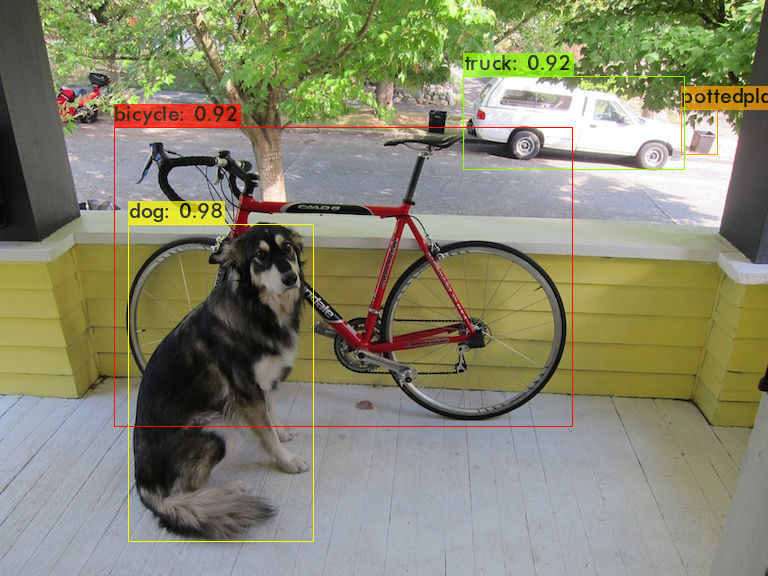
\includegraphics[width=\textwidth]{img/chapters/desarrollo/predictions.jpg}
    \caption{}
    \label{fig:predictions-darknet}
  \end{subfigure}
  \qquad\qquad
  \begin{subfigure}[b]{0.4\textwidth}
    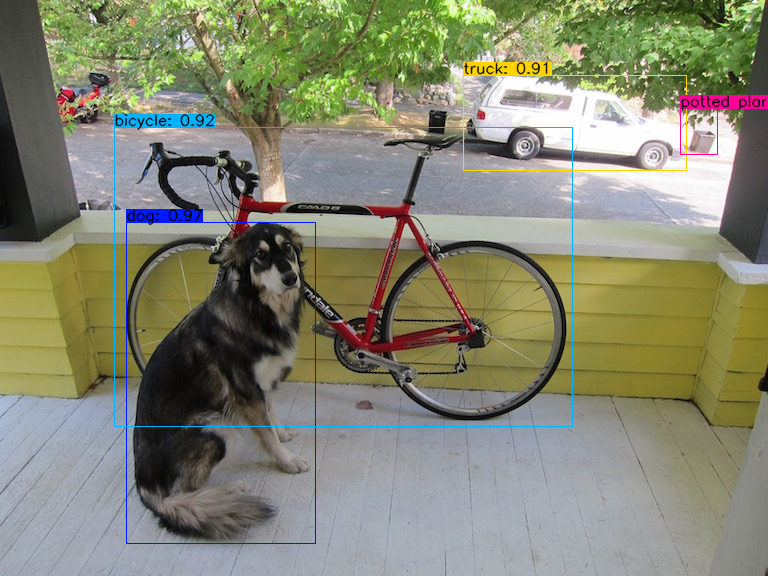
\includegraphics[width=\textwidth]{img/chapters/desarrollo/detection1.png}
    \caption{}
    \label{fig:predictions-tf}
  \end{subfigure}
  \caption{Detecciones de YOLOv4 con Darknet y Tensorflow.
    (\protect\subref{fig:predictions-darknet}) Detección de YOLOv4 con Darknet.
    (\protect\subref{fig:predictions-tf}) Detección de YOLOv4 con Tensorflow.}
  \label{fig:predictions-darknet-tf}
\end{figure}

\newpage

\section{Datasets utilizados para el evaluación de YOLOv4}
\label{sec:datasets-utilizados}

\textcolor{red}{Hacer introducción y ajustar imágenes de esta sección antes de seguir con la siguiente}

asdfasdf

asdfasdf

asdfasdf

asdfasdf

asdfasdf

asdfasdf

asdfasdf

asdfasdf

\subsection{MS COCO Dataset}
\label{subsec:coco-dataset}

El dataset \gls{coco} \cite{lin2015microsoft} es un conjunto de datos de referencia utilizado para evaluar el rendimiento de los modelos entrenados por visión por computadora. Está diseñado para representar una amplia gama de objetos que encontramos regularmente en la vida cotidiana.

\begin{figure}[ht]
\centering
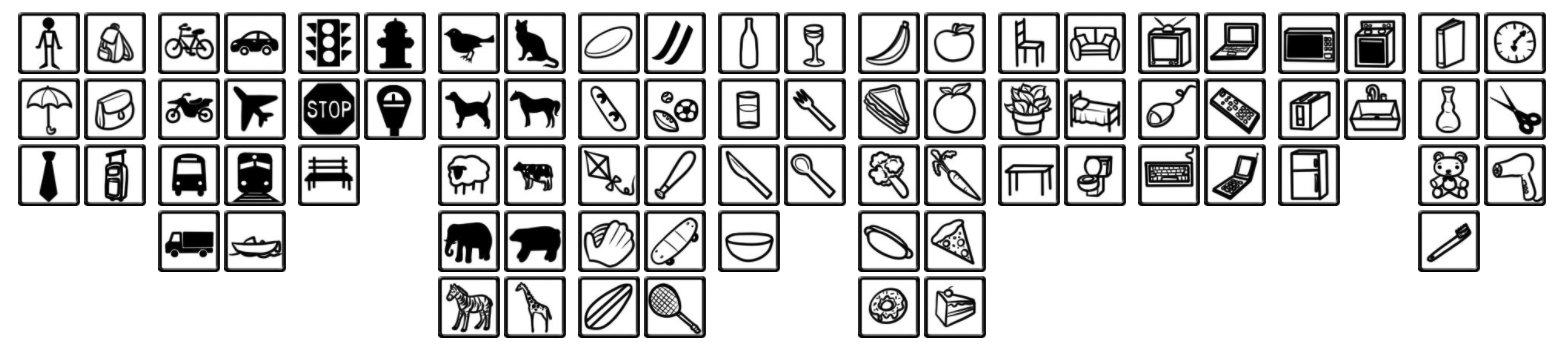
\includegraphics[width=0.9\textwidth]{img/chapters/desarrollo/cocodataset.png}
\caption{\label{fig:cocodataset}Categorías de objetos del dataset MS COCO \cite{coco-official-website}}
\end{figure}

\gls{coco} está etiquetado en un formato especial llamado COCO JSON, y proporciona datos para entrenar modelos supervisados de visión por computadora que son capaces de identificar los objetos comunes del conjunto de datos. Estos modelos están lejos de ser perfectos, por lo que el dataset \gls{coco} proporciona un punto de referencia para evaluar la mejora periódica de estos modelos a través de la investigación en visión por computadora.

Otra motivación para el dataset \gls{coco} es proporcionar un conjunto de datos base para entrenar modelos de visión por computadora. Una vez entrenado el modelo, se puede perfeccionar para aprender otras tareas, como datasets personalizados.

\subsubsection*{Tareas de MS COCO}
\label{subsubsec:tareas-coco}

\gls{coco} tiene múltiples tareas de visión por computadora. A continuación, se enumeran en orden decreciente en base a su uso:

\begin{itemize}
    \item \textbf{Detección de objetos}: los objetos se anotan con un cuadro delimitador y una etiqueta de clase. El dataset \gls{coco} tiene 121.408 imágenes para detección de objetos, 883.331 anotaciones de objetos, 80 clases (ver figura \ref{fig:cocodataset}) y una resolución media de imagen de 640x480.
    
    \begin{figure}[ht]
    \centering
    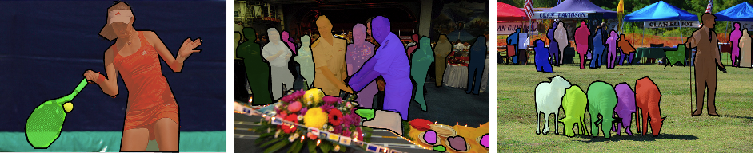
\includegraphics[width=0.65\textwidth]{img/chapters/desarrollo/detection-splash.png}
    \caption{\label{fig:detection-splash}MS COCO detección de objetos \cite{coco-official-website}}
    \end{figure}
    
    \item \textbf{Segmentación semántica}: los límites de los objetos se etiquetan con una máscara y las clases de objetos se etiquetan con una etiqueta de clase. La segmentación semántica requiere modelos para trazar los límites entre los objetos.
    
    \begin{figure}[ht]
    \centering
    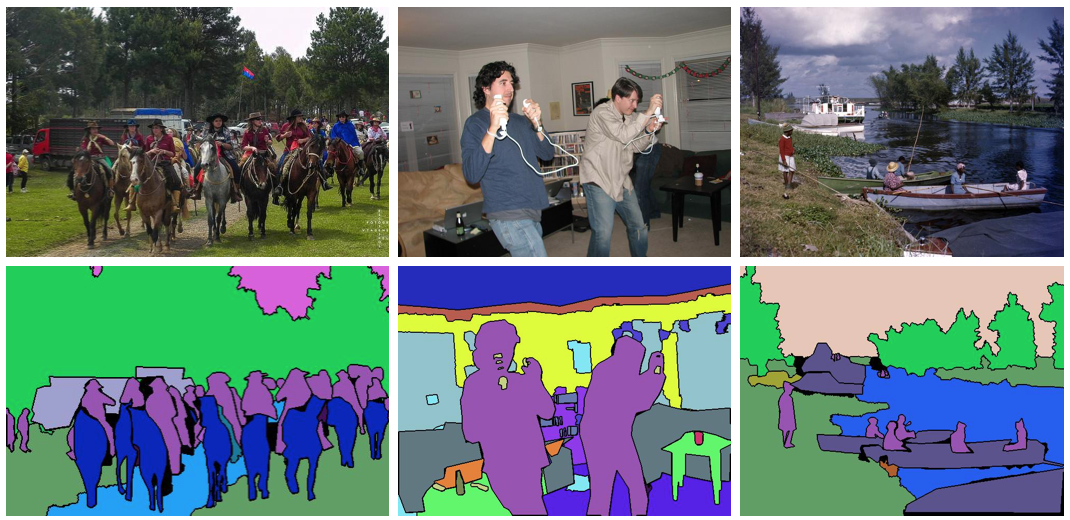
\includegraphics[width=0.6\textwidth]{img/chapters/desarrollo/panoptic-splash.png}
    \caption{\label{fig:panoptic-splash}MS COCO segmentación semántica \cite{coco-official-website}}
    \end{figure}    
    
    \item \textbf{Detección de puntos clave}: las personas son etiquetadas con puntos claves de interés (como pueden ser codos, rodillas o cabezas). El dataset \gls{coco} dispone de 250.000 personas con puntos clave etiquetados.
    
    \begin{figure}[ht]
    \centering
    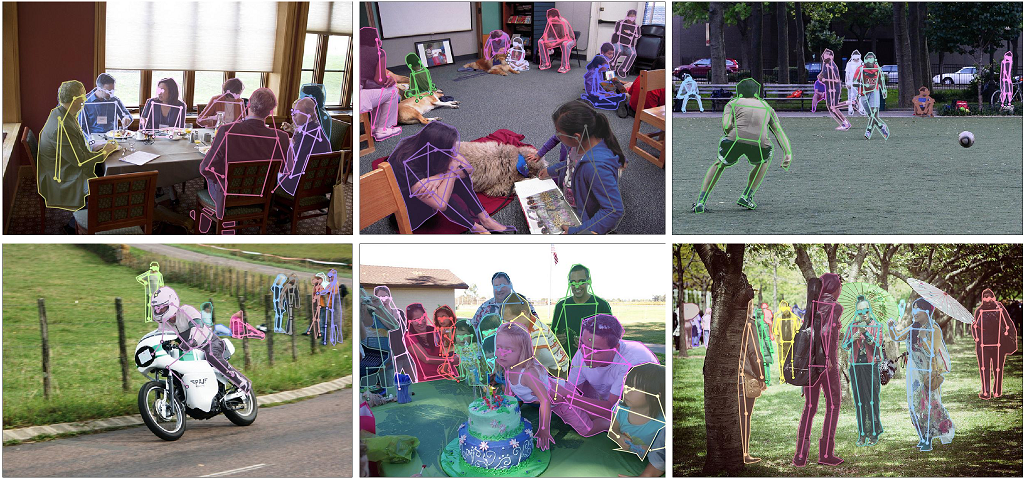
\includegraphics[width=0.6\textwidth]{img/chapters/desarrollo/keypoints-splash-big.png}
    \caption{\label{fig:keypoints-splash-big}MS COCO detección de puntos clave \cite{coco-official-website}}
    \end{figure}    
    
\end{itemize}

\subsection{Open Images Dataset v4}
\label{subsec:OIDv4-dataset}

\gls{oidv4} \cite{Kuznetsova_2020} es un conjunto de datos de 9,2 millones de imágenes con anotaciones en formato .txt unificadas para la clasificación de imágenes, detección de objetos y detección de relaciones visuales (ver figura \ref{fig:example-annotations-oidv4}). Las imágenes tienen una licencia Creative Commons Attribution que permite compartir y adaptar el material descargado de Flickr sin una lista predefinida de nombres de clases o etiquetas.

\begin{figure}[ht]
\centering
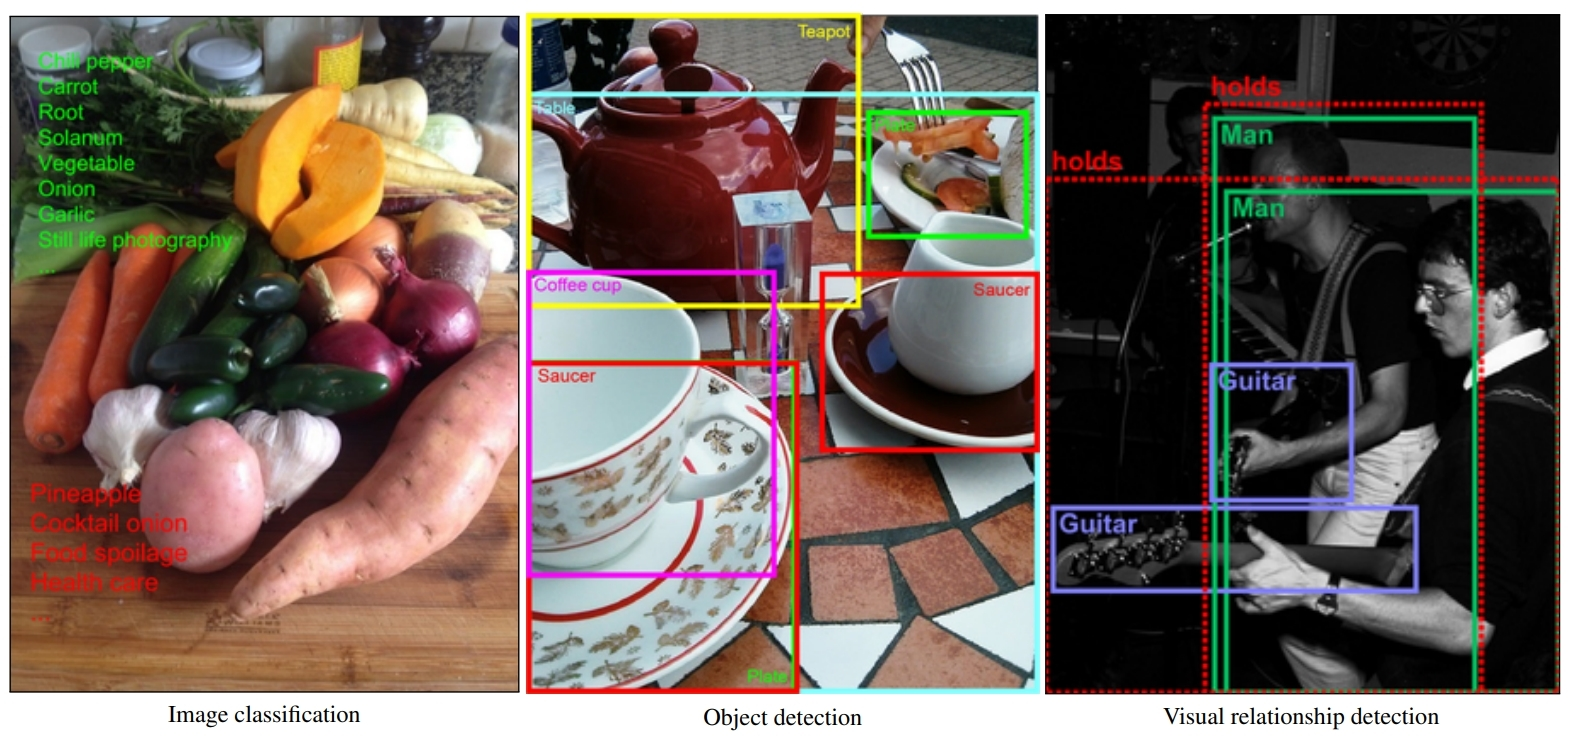
\includegraphics[width=0.6\textwidth]{img/chapters/desarrollo/example-annotations-oidv4.jpg}
\caption{\label{fig:example-annotations-oidv4}Ejemplo anotaciones en Open Images Dataset v4 \cite{Kuznetsova_2020}}
\end{figure}

\gls{oidv4} ofrece una gran escala en varias dimensiones: 30,1 millones de etiquetas a nivel de imagen para 19,8 mil conceptos, 15,4 millones de cuadros delimitadores para las 600 clases de objetos que se muestran en la figura \ref{fig:oidv4dataset}, y 375 mil anotaciones de relaciones visuales que involucra 57 clases. Para la detección de objetos se proporciona más de 15 veces cuadros delimitadores que otros grandes datasets como \gls{coco} o ImageNet. Las imágenes suelen mostrar escenas complejas con varios objetos (de promedio tiene 8 objetos anotados por imagen). 

\begin{figure}[ht]
\centering
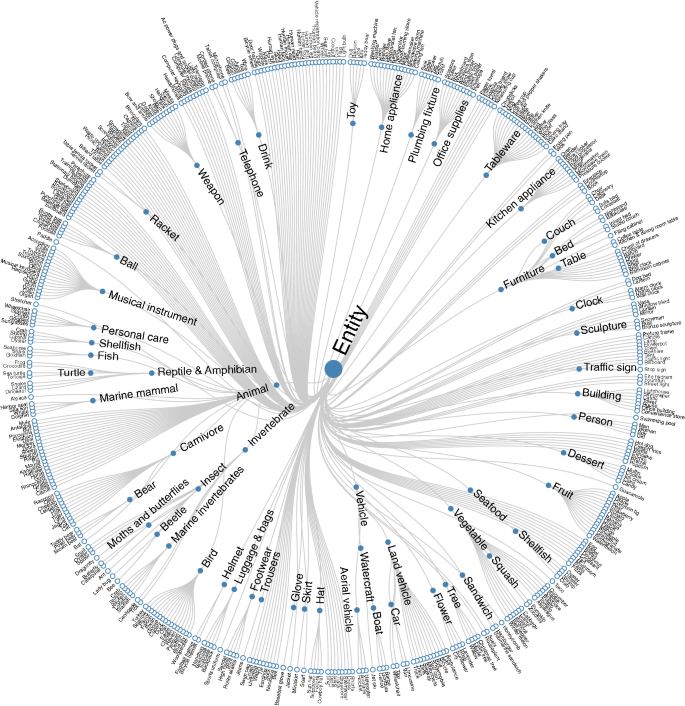
\includegraphics[width=0.65\textwidth]{img/chapters/desarrollo/oidv4-classes.png}
\caption{\label{fig:oidv4dataset}Categorías de objetos del dataset Open Images Dataset v4 \cite{Kuznetsova_2020}}
\end{figure}

\section{Evaluación de las métricas de calidad de MS COCO dataset}
\label{sec:evaluate-cocodataset}

En está sección se va a evaluar las métricas de calidad del dataset \gls{coco} para tener una referencia a la hora de valorar, si reentrenando la red, se pueden obtener mejores métricas para la aplicación del proyecto.

Primero se ha descargado el repositorio oficial de \gls{yolov4} de GitHub \cite{yolov4-darknet-github}. Para aprovechar maximizar la eficiencia de la evaluación se ha modificado el fichero Makefile para habilitar la \gls{gpu} junto con \gls{cuda} y OpenCV. En esta evaluación se ha utilizado una NVIDIA Tesla T4, por lo que ha sido necesario especificar que se va a utilizar una \gls{gpu} con una capacidad de cálculo de 7,5.

\vspace{0.5cm}
\begin{lstlisting}[language=iPython,caption=Evaluación de las métricas de calidad de MS COCO en YOLOv4 Darknet (1),captionpos=b,label={lst:evaluate-cocodataset1}]
# Clonar el repositorio de GitHub de YOLOv4 darknet
git clone https://github.com/AlexeyAB/darknet

# Entrar dentro de la carpeta del repositorio
cd darknet

# Modificar las siguientes lineas del fichero makefile para habilitar la GPU y OPENCV
sed -i 's/OPENCV=0/OPENCV=1/' Makefile
sed -i 's/GPU=0/GPU=1/' Makefile
sed -i 's/CUDNN=0/CUDNN=1/' Makefile
sed -i 's/CUDNN_HALF=0/CUDNN_HALF=1/' Makefile
sed -i 's/# ARCH= -gencode arch=compute_75/ARCH= -gencode arch=compute_75/' Makefile

# Compilar mediante el comando make
make
\end{lstlisting}

Dentro de la carpeta del repositorio se ha creado una carpeta llamada \texttt{images} donde se almacenarán las imágenes del entrenamiento y validación del modelo de \gls{yolov4}. Tal y como se muestra en el código \ref{lst:evaluate-cocodataset2} se han descargado los ficheros comprimidos de las imágenes desde la web oficial de \gls{coco} \cite{coco-official-website}.

\vspace{0.5cm}
\begin{lstlisting}[language=iPython,caption=Evaluación de las métricas de calidad de MS COCO en YOLOv4 Darknet (2),captionpos=b,label={lst:evaluate-cocodataset2}]
# Crear y entrar en la carpeta ./images donde descargaremos las imagenes
mkdir images
cd images

# Descargar, descomprimir y borrar archivo comprimido .zip de las imagenes de entrenamiento
wget -c http://images.cocodataset.org/zips/train2017.zip
unzip -q train2017.zip
rm train2017.zip

# Descargar, descomprimir y borrar archivo comprimido .zip de las imagenes de validacion
wget -c http://images.cocodataset.org/zips/val2017.zip
unzip -q val2017.zip
rm val2017.zip

# Vuelta a la carpeta raiz
cd ..
\end{lstlisting}

En el siguiente \href{https://drive.google.com/drive/folders/1KLf2PTMwPmopPxPdFLtx-nAPpdlcT-NF?usp=sharing}{link} se encuentran los ficheros \texttt{train2017.txt} y \texttt{val2017.txt}, que contienen las rutas donde se encuentran almacenadas las imágenes de entrenamiento y validación, y copiarlas dentro de la carpeta \texttt{./data}. Por otro lado, se han copiado los ficheros de las etiquetas de las imágenes de entrenamiento que se encuentran dentro de la carpeta comprimida \texttt{./labels/train2017} y pegado dentro de la carpeta \texttt{./images/train2017} del repositorio. Del mismo modo, se han copiado los ficheros de las etiquetas de las imágenes de entrenamiento que se encuentran dentro de la carpeta comprimida \texttt{./labels/val2017} y pegado dentro de la carpeta \texttt{./images/val2017} del repositorio.

Es necesario modificar el fichero que se encuentran en \texttt{./cfg/coco.data} para especificar por un lado, el número de clases que tiene el modelo que se quiere evaluar (no se ha tocado ya porque viene por defecto las 80 clases que componen el dataset \gls{coco}), la ubicación de los ficheros \texttt{train2017.txt} y \texttt{val2017.txt} y el fichero coco.names que contiene el nombre de cada una de las 80 clases.

\vspace{0.5cm}
\begin{lstlisting}[language=iPython,caption=Fichero coco.data,captionpos=b,label={lst:coco-data-file}]
classes = 80
train  = data/train2017.txt
valid  = data/val2017.txt
names = data/coco.names
#backup = /home/pjreddie/backup/
\end{lstlisting}

Por último, se han descargado los pesos del modelo de \gls{yolov4} preentrado y ejecutado el siguiente comando para evaluar las métricas de calidad en base al dataset \gls{coco}.

\vspace{0.5cm}
\begin{lstlisting}[language=iPython,caption=Evaluación de las métricas de calidad de MS COCO en YOLOv4 Darknet (3),captionpos=b,label={lst:evaluate-cocodataset3}]
# Descargar los pesos preentrenados de YOLOv4
wget https://github.com/AlexeyAB/darknet/releases/download/darknet_yolo_v3_optimal/yolov4.weights

# Ejecutar evaluacion de las metricas de calidad de MS COCO sobre YOLOv4
./darknet detector map ./cfg/coco.data ./cfg/yolov4.cfg ./yolov4.weights
\end{lstlisting}

En la sección \ref{subsec:metricas-calidad-coco} se expondrán los resultados obtenidos tras la evaluación de las métricas de calidad.

Se ha creado un Notebook de Google Colab para la evaluación de las métricas de calidad de \gls{coco}. Se puede acceder entrando en este \href{https://colab.research.google.com/drive/19P6tIicaeD9vOTCl42eI9PR1nXVlsfoH?usp=sharing}{link}.

\aviso{Mostrar imágenes de los resultados explicando por encima los resultados que se obtienen, explicar un poco más por encima esta parte y finalmente decir que en secciones futuras (resultados) se analizará con más detalle los valores obtenidos en el dataset MS COCO}

\section{Entrenamiento YOLOv4 con Open Image Dataset v4}
\label{sec:train-openimagesv4}

\subsection{Recopilación y etiquetado del dataset personalizado}
\label{subsec:recopilacion-etiquetado-custom-dataset}

\textcolor{red}{Aquí explicar como he entrenado una red neuronal con otro dataset a partir del repositorio \cite{OIDv4_ToolKit}}

\textcolor{red}{Explicar que se ha tomado 1.500 imágenes de entrenamiento de las clases: person, handbag, backpack, suitcase y 300 imágenes de validación.}

\textcolor{red}{Explicar también que, tal y como se ven en la seccion XXX de los resultados, resulta interesante probar a reentrenar la red para ver si se pueden mejorar las metricas de calidad.}

\vspace{0.5cm}
\begin{lstlisting}[language=iPython,caption=Descarga dataset Open Images Dataset v4 (1),captionpos=b,label={lst:download-oidv4_1}]
# Clonar el repositorio de Github
git clone https://github.com/theAIGuysCode/OIDv4_ToolKit.git
cd OIDv4_ToolKit

# Instalacion de las librerias y dependendencias (recomendable crear un entorno virtual con Anaconda)
pip install -r requirements.txt
\end{lstlisting}

\vspace{0.5cm}
\begin{lstlisting}[language=iPython,caption=Descarga dataset Open Images Dataset v4 (2),captionpos=b,label={lst:download-oidv4_2}]
# Descarga de las imagenes de entrenamiento con un limite de 1500
python main.py downloader --classes Person Handbag Backpack Suitcase --type_csv train --limit 1500 --multiclasses 1

# Descarga de las imagenes de validacion con un limite de 300
python main.py downloader --classes Person Handbag Backpack Suitcase --type_csv validation --limit 300 --multiclasses 1
\end{lstlisting}



\begin{figure}[ht]
\centering
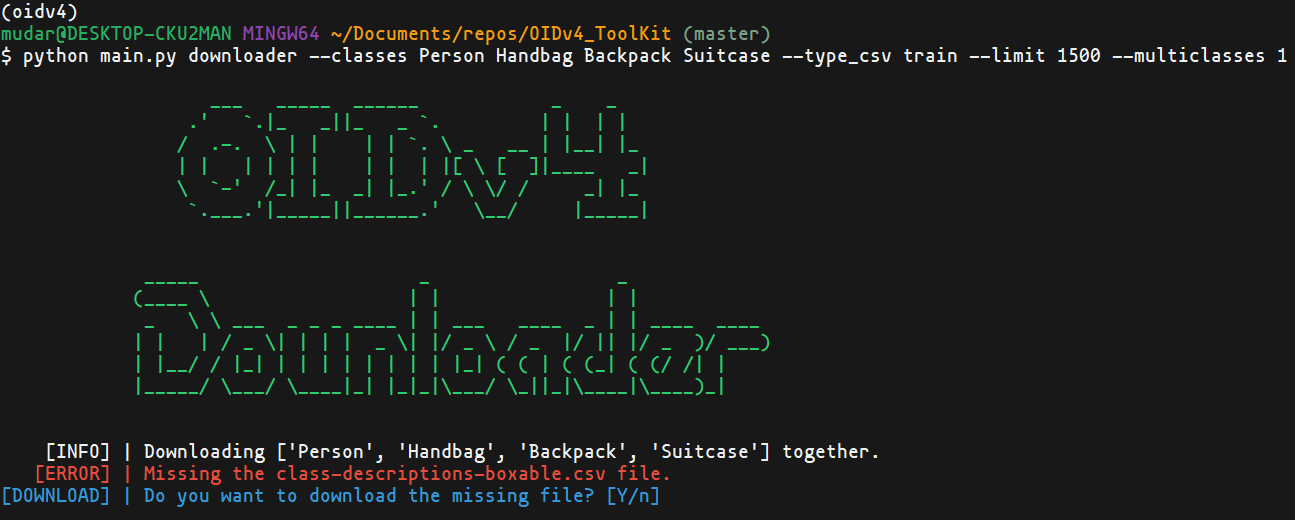
\includegraphics[width=0.75\textwidth]{img/chapters/resultados/datasets/download-oidv4.png}
\caption{\label{fig:download-oidv4}Descarga del dataset Open Images Dataset v4}
\end{figure}

\begin{figure}[ht]
\centering
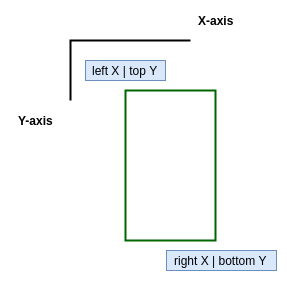
\includegraphics[width=0.45\textwidth]{img/chapters/resultados/datasets/bbox-oidv4.png}
\caption{\label{fig:bbox-oidv4}Estructura de las etiquetas de Open Images Dataset v4 \cite{OIDv4_ToolKit}}
\end{figure}



La estructura que siguen las etiquetas del dataset de Open Images Dataset v4 es la siguiente:

\texttt{nombre\_de\_la\_clase left\_x top\_y right\_x bottom\_y}

Las etiquetas que se obtienen mediante esta herramienta no tienen el mismo formato que Darknet. Afortunadamente, el repositorio \cite{OIDv4_ToolKit} dispone del script \texttt{convert\_annotations.py} para convertir el etiquetado tanto de las imágenes de entrenamiento como las de validación del dataset \gls{oidv4} a Darknet. Antes de su ejecución, se han sustituido en el fichero \texttt{classes.txt} las clases que habían por defecto por el nombre de las clases que se han descargado imágenes en el mismo orden que cuando se nombraron en el código \ref{lst:download-oidv4_2}, para que la conversión se realice correctamente. Después se puede ejecutar la siguiente línea de código:

\vspace{0.5cm}
\begin{lstlisting}[language=iPython,caption=Descarga dataset Open Images Dataset v4 (3),captionpos=b,label={lst:download-oidv4_3}]
# Convertir etiquetas al formato de Darknet
python convert_annotations.py
\end{lstlisting}

Al finalizar la conversión de las etiquetas, se han borrado las carpetas \texttt{Label} que contienen el etiquetado en el formato original. Las carpetas \texttt{obj} y \texttt{test} se han copiado a la carpeta \texttt{./data} del repositorio de \gls{yolov4} con Darknet que se explicó en la sección \ref{sec:desarrollo-yolov4}, donde se realizará el entrenamiento del modelo en base al dataset personalizado.

\subsection{Configuración de ficheros para el entrenamiento}
\label{subsec:configuracion-ficheros-training}

Se ha hecho una copia de \texttt{yolov4.cfg} con nombre \texttt{yolov4-obj.cfg} y se ha modificado los siguientes parámetros en base a las recomendaciones indicadas en el apartado de entrenamiento de datasets personalizados de \cite{yolov4-darknet-github}:

\begin{itemize}
    \item \texttt{width} = \texttt{weight} = 416 (Tamaño estándar para probar en el primer entrenamiento)
    \item \texttt{max\_batches} = (\# de clases) * 2.000 = 4 * 2.000 = 8.000
    \item \texttt{steps} = 6.400 (80\% de max\_batches), 7.200 (90\% de max\_batches)
    \item \texttt{filters} = (\# de clases + 5) * 3 = (4 + 5) * 3 = 27
\end{itemize}

\vspace{0.5cm}
\begin{lstlisting}[language=iPython,caption=Fichero obj.data,captionpos=b,label={lst:obj-data-file}]
classes = 4
train = data/train.txt
valid = data/test.txt
names = data/obj.names
backup = /mydrive/yolov4/backup
\end{lstlisting}

\vspace{0.5cm}
\begin{lstlisting}[language=iPython,caption=Fichero obj.names,captionpos=b,label={lst:obj-names-file}]
Person
Handbag
Backpack
Suitcase
\end{lstlisting}

\vspace{0.5cm}
\begin{lstlisting}[language=iPython,caption=Generación train.txt y test.txt,captionpos=b,label={lst:train-test-generate}]
import os

image_files = []
os.chdir(os.path.join("data", "obj"))
for filename in os.listdir(os.getcwd()):
    if filename.endswith(".jpg"):
        image_files.append("data/obj/" + filename)
os.chdir("..")
with open("train.txt", "w") as outfile:
    for image in image_files:
        outfile.write(image)
        outfile.write("\n")
    outfile.close()
os.chdir("..")
\end{lstlisting}

Para las imágenes de validación hacer exactamente el mismo procedimiento sustituyendo \texttt{test} por \texttt{obj} en el código \ref{lst:train-test-generate}.

\subsection{Entrenamiento del dataset personalizado}
\label{subsec:training-custom-dataset}

\vspace{0.5cm}
\begin{lstlisting}[language=iPython,caption=Entrenamiento del dataset personalizado,captionpos=b,label={lst:training-custom-dataset}]
# Descarga de los pesos pre-entrenados para las capas convolucionales
wget https://github.com/AlexeyAB/darknet/releases/download/darknet_yolo_v3_optimal/yolov4.conv.137

# Comenzar a entrenar la red neuronal del dataset personalizado de OIDv4
./darknet detector train data/obj.data cfg/yolov4-obj.cfg yolov4.conv.137 -dont_show -map
\end{lstlisting}

\newpage

\section{Seguimiento de personas y objetos con YOLOv4 y Deep SORT}
\label{sec:desarrollo-yolov4+deepsort}

\textcolor{red}{Aquí hacer una breve descripción de deepsort, muy breve porque ya se ha explicado en el capitulo del estado del arte, y poner imagenes de su funcionamiento sobre yolov4 en el framework tensorflow}.

\textcolor{red}{Dado que el código que se va a comentar en esta sección es bastante largo para reflejarlo se ha optado por crear un apéndice al final del documento dedicado al mismo}.

\textcolor{red}{Se utilizará el mismo entorno virtual que el de detección de objetos con YOLOv4 en Tensorflow}

\vspace{0.5cm}
\begin{lstlisting}[language=iPython,caption=Evaluación del seguimiento de objetos Deep SORT y YOLOv4 en Tensorflow (1),captionpos=b,label={lst:evaluate-deepsort-tf1}]
# Descarga del repositorio de GitHub
git clone https://github.com/jmudy/yolov4-deepsort

# Entrar dentro de la carpeta del repositorio
cd yolov4-deepsort

# Cambiar a la rama de git develop y comprobar que nos encontramos en ella
git checkout develop
git branch -a

# Descarga de los pesos de YOLOv4
wget https://github.com/AlexeyAB/darknet/releases/download/darknet_yolo_v3_optimal/yolov4.weights -P ./data/
\end{lstlisting}

\textcolor{red}{bla bla bla}

\vspace{0.5cm}
\begin{lstlisting}[language=iPython,caption=Evaluación del seguimiento de objetos Deep SORT y YOLOv4 en Tensorflow (2),captionpos=b,label={lst:evaluate-deepsort-tf2}]
# Ejecutar algoritmo de seguimiento de objetos con Deep SORT y YOLOv4 en Tensorflow
!python object_tracker.py --video {input_file_name.mp4} --output {output_file_name.avi} --model yolov4 --size 608 --weights ./checkpoints/yolov4-608 --count --info
\end{lstlisting}


\newpage

\section{Algoritmo de detección de objetos abandonados}
\label{sec:algoritmo-object-detection}

\textcolor{red}{Dibujar el esquema que voy a seguir para determinar cuando un objeto ha sido abandonado.}
\url{https://app.diagrams.net/}

\textcolor{red}{Intentar meter toda la chicha posible. Que quede pendiente meter aquí código de lo que he implementado para que no quede todo en el aire y se vean de repente los resultados, por lo menos que se vea la función que hace la asociación de persona objeto y la función que establece si la persona ha abandonado un objeto o si el objeto esta abandonado y sin propietario.}

\textcolor{red}{Poner figura ejemplo de la hipotesis donde se hace asociacion de persona y objeto cuando se activa la alarma y cuando se determina que un objeto ha sido abandonado, en el momento de la alarma se ejecuta una cuenta atrás de 30 segundos antes de determinar que el objeto ha sido abandonado.}

\textcolor{red}{Explicar la hipótesis de cuando un objeto no tiene propietario porque se encuentra alejado de cualquier persona en los primeros fotogramas del vídeo. En este caso al pasar 15 segundos se determina que el objeto ha sido abandonado.}

Cuando se calcula se calcula la distancia entre personas y objetos de interés se calcula la media de las distancias obtenidas fotograma a fotograma en los primeros 5 segundos de vídeo. Se crea una asociación de una persona al objeto que se haya obtenido la menor distancia en el momento de la asociación, siempre y cuando esa distancia sea inferior a dos veces el ancho del cuadro limitador del objeto, para así no depender de la profundidad a la que se pueda encontrar las personas y objetos dentro del plano de visión.

\begin{figure}[ht]
\centering
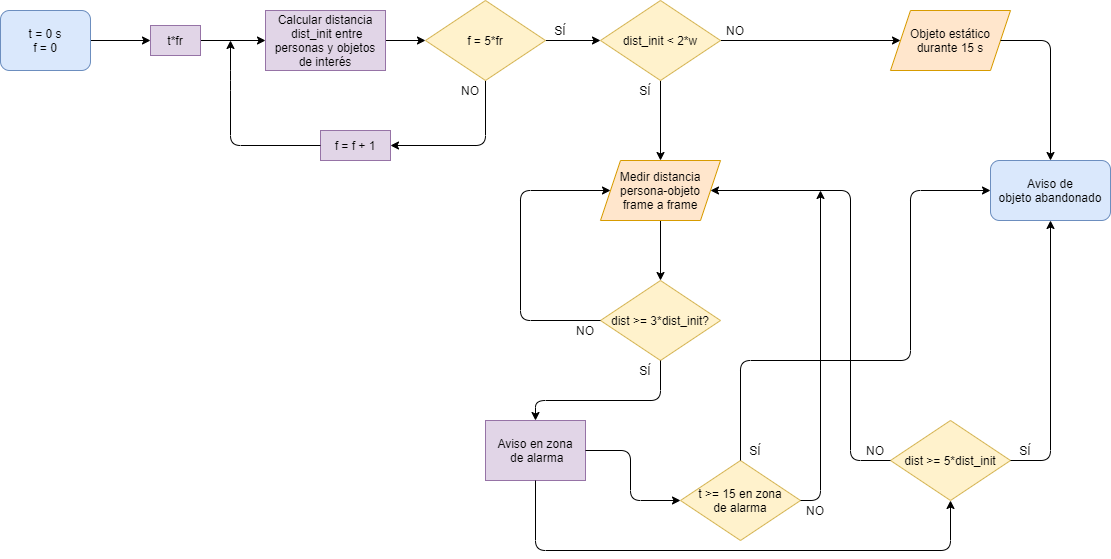
\includegraphics[width=1\textwidth]{img/chapters/desarrollo/abandoned-object-scheme.png}
\caption{\label{fig:abandoned-object-scheme}Esquema hipótesis detección objeto abandonado}
\end{figure}

\newpage

\begin{figure}[ht]
\centering
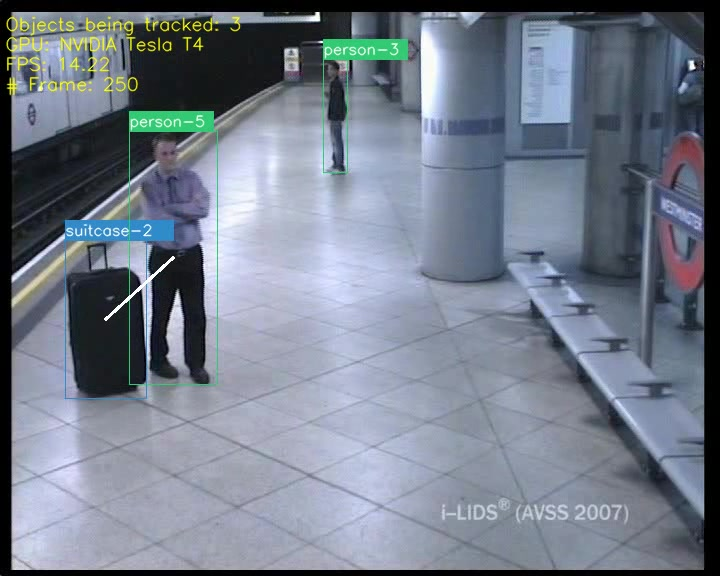
\includegraphics[width=0.4\textwidth]{img/chapters/desarrollo/link-persona-objeto.jpg}
\caption{\label{fig:link-persona-objeto}Asociación persona-objeto}
\end{figure}

Hola hola

\begin{figure}[ht]
\centering
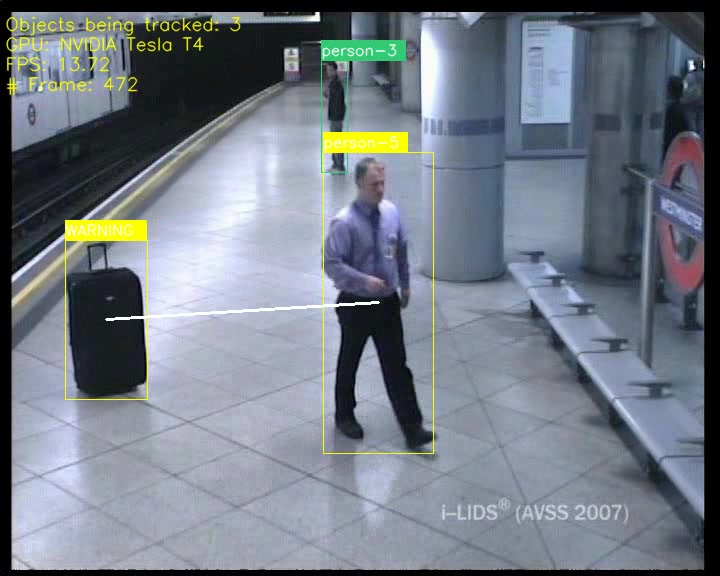
\includegraphics[width=0.4\textwidth]{img/chapters/desarrollo/warning-abandono.jpg}
\caption{\label{fig:warning-abandono}Aviso de alerta posible objeto abandonado}
\end{figure}

Hola hola

\begin{figure}[ht]
\centering
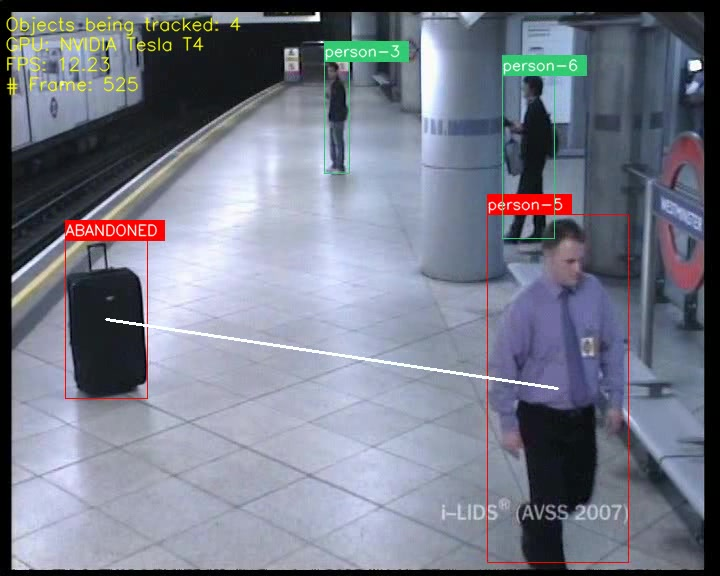
\includegraphics[width=0.4\textwidth]{img/chapters/desarrollo/abandono-objeto-avss.jpg}
\caption{\label{fig:abandono-objeto-avss}Detección de objeto abandonado}
\end{figure}

Hola hola

\newpage

\vspace{0.5cm}
\begin{lstlisting}[language=iPython,caption=Evaluación de la detección de objetos abandonados con DeepSORT y YOLOv4 en Tensorflow (1),captionpos=b,label={lst:evaluate-abandoned-object1}]
# Descarga del repositorio de GitHub
git clone https://github.com/jmudy/yolov4-deepsort

# Entrar dentro de la carpeta del repositorio
cd yolov4-deepsort

# Cambiar a la rama de git abandoned y comprobar que nos encontramos en ella
git checkout abandoned
git branch -a

# Descarga de los pesos de YOLOv4
wget https://github.com/AlexeyAB/darknet/releases/download/darknet_yolo_v3_optimal/yolov4.weights -P ./data/
\end{lstlisting}

\textcolor{red}{bla bla bla}

\vspace{0.5cm}
\begin{lstlisting}[language=iPython,caption=Evaluación de la detección de objetos abandonados con DeepSORT y YOLOv4 en Tensorflow (2),captionpos=b,label={lst:evaluate-abandoned-object2}]
# Ejecutar algoritmo de deteccion objetos abandonados con Deep SORT y YOLOv4 en Tensorflow
!python abandoned_object.py --video {input_file_name.mp4} --output {output_file_name.avi} --model yolov4 --size 608 --weights ./checkpoints/yolov4-608 --count --info
\end{lstlisting}


\newpage

\section{Conclusiones}
\label{sec:conclu-desarrollo}

\textcolor{red}{Hacer unas breves conclusiones de lo que se ha conseguido en base a los objetivos que se han marcado en la introducción de este capítulo \ldots}

\begin{algorithm}[H]
 \caption{How to write algorithms}
 \label{alg:howto}
 \KwData{this text}
 \KwResult{how to write algorithm with \LaTeX}
 initialization\;
 \While{not at end of this document}{
  read current\;
  \eIf{understand}{
   go to next section\;
   current section becomes this one\;
   }{
   go back to the beginning of current section\;
  }
 }
\end{algorithm}